\chapter{Descripción del Proyecto}\label{cap:01introduccion}

Este primer capítulo del Trabajo Fin de Grado (TFG) se divide en cinco secciones: \ref{sec:01intro} Introducción, \ref{sec:01Contexto} Contexto, \ref{sec:01EstadoArte} Estado del arte, \ref{sec:01Motivacion} Motivación y \ref{sec:01estructura} Estructura de la memoria.

\section{Introducción} \label{sec:01intro}

El proyecto consiste en el \textbf{\textit{\tfgTitle}} a través de la realización de un estudio teórico exhaustivo de la organización Observational Health Data Sciences and Informatics (OHDSI) y la aplicación de un caso práctico utilizando la herramienta de análisis de datos ATLAS.

Los contenidos de este capítulo consisten principalmente en la descripción del panorama sanitario y tecnológico actual, de especial relevancia para conocer la importancia de la organización OHDSI en el contexto que envuelve a la informática clínica actual.

En la sección \ref{sec:01Contexto} ''Contexto'' se presentan las características de la Sanidad 4.0 y los desafíos del sector en paralelo a las propuestas más relevantes que introduce OHDSI para paliar estas dificultades.

En la sección \ref{sec:01EstadoArte} ''Estado del arte'' se presentan las alternativas a OHDSI más empleadas actualmente a nivel global en términos de estandarización y herramientas de análisis de datos clínicos.

Por último, en la sección \ref{sec:01Motivacion} ''Motivación'' se presenta la motivación personal de la alumna para realizar el proyecto y la colaboración con el Hospital Universitario Virgen del Rocío en esta labor y en la sección \ref{sec:01estructura} ''Estructura de la memoria'' se expone brevemente la estructura seguida a lo largo de la memoria y los contenidos que se tratan en la misma, incluyendo los anexos.


\section{Contexto} \label{sec:01Contexto} 
%Intención: dar a conocer al lector los aspectos y características fundamentales del panorama sanitario y tecnológico actual, necesario para comprender en profundidad el trabajo.

El contexto en el que se desarrolla el proyecto se caracteriza por el impacto transformador de la Industria 4.0 y las tecnologías que la acompañan en el sector sanitario, que dan lugar a la Sanidad 4.0. De este nuevo paradigma tecnológico-sanitario emergen nuevas necesidades de interoperabilidad entre los sistemas informáticos y desafíos en el tratamiento de la información sanitaria.

Frente a ello, la organización OHDSI se levanta como una solución innovadora y potente para paliar las necesidades de la industria. A continuación, en la Figura \ref{fig:esquemaMarcoContextual} se presenta un flujo sencillo de los contenidos que se desarrollan esta sección.

\begin{figure}[H]
    \centering
    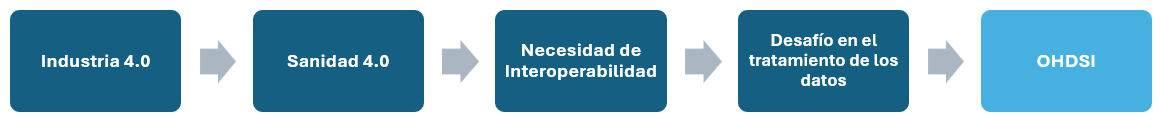
\includegraphics[width=1\textwidth]{figures/esquemaMarcoContextual.png}
    \caption{Esquema de contenidos de la sección \ref{sec:01Contexto} ''Contexto''}
    \label{fig:esquemaMarcoContextual}
\end{figure}


\subsubsection{1.2.1 La Industria 4.0 y las tecnologías emergentes}

La Industria 4.0, o cuarta revolución industrial, fue un concepto concebido por el gobierno alemán en noviembre de 2011. Nace como una estrategia tecnológica para abordar el crecimiento industrial proyectado para 2020 y representa la cuarta fase de la industrialización, sucediendo a la mecanización, electrificación e informatización, y destaca la integración digital de tecnologías avanzadas \parencite{lasi2014industry}.

Dicho concepto se centra principalmente en la digitalización y la necesaria convergencia entre los sistemas físicos y los sistemas cibernéticos (\textit{Cyber-Physical Systems, CPS}). Esta integración se busca mediante el despliegue  de nuevas tecnologías de la información y telecomunicación (TICs), como el tan sonado internet de las cosas (\textit{Internet of Things, IoT}), la generación y análisis de datos masivos (\textit{Big Data \& Big Data Analytics}), la computación en la nube (\textit{Cloud Computing}) y el tremendo auge de la Inteligencia Artificial (IA) \parencite{lasi2014industry, chen2020times, tortorella2020healthcare}

\subsubsection{1.2.2 Características de la Sanidad 4.0}

La integración de los principios y tecnologías de la Industria 4.0 en el sector sanitario originó el concepto de Salud o Sanidad 4.0 (\textit{Healthcare 4.0}) \parencite{tortorella2020healthcare, tortorella2021impacts}. 
Esto origina un nuevo paradigma del que se destacan a continuación tres características principales: %(i) la provisión continua de cuidado sanitario, (ii) la orientación de la medicina hacia el paciente y (iii) la prevención y predicción de enfermedades. A continuación se describe cada una esta de estas características:

\begin{itemize}

\item \textbf{Cuidado sanitario continuo (\textit{continuum of care})}. Las tecnologías TIC y el IoT, han permitido a la sociedad estar altamente conectada, lo que ha impulsado el desarrollo de la telemedicina y la e-Salud, especialmente tras la pandemia del COVID-19 \parencite{martin2021ehealth}. Se han desarrollado numerosos dispositivos portátiles, como pulseras y relojes inteligentes, para monitorear a los pacientes de forma continua tanto dentro como fuera del entorno hospitalario. Estos dispositivos generan de forma casi ininterrumpida grandes cantidades de datos médicos que se combinan con registros clínicos para formar los llamados 'Datos del mundo real' \textit{(Real World Data, RWD)} \parencite{kouroubali2019new}. 

La gestión de estas grandes y dispares cantidades de información es una tarea muy compleja. Usualmente los datos se recopilan de distintas formas según su finalidad. OHDSI tiene como objetivo poner fin a la disparidad estructural de la información sanitaria proveyendo un modelo de datos común que permita recopilar los datos con fines observacionales.

\item \textbf{Centrada en el paciente}. Esta perspectiva enfatiza al paciente como el eje central de la atención sanitaria \parencite{tortorella2020healthcare}. Con el avance de la medicina de precisión y el seguimiento remoto de la actividad diaria, la atención médica se ha vuelto cada vez más personalizada \parencite{ruiz2023inteligencia}. La Unión Europea promueve esta orientación, exigiendo una reestructuración del sistema sanitario para que el paciente sea el principal beneficiario, evaluador y centro de los servicios de salud digital \parencite{ntafi2022legal, katehakis2019framework}. Esto implica la implementación de sistemas informáticos que administren el historial clínico electrónico (HCE) completo de cada individuo, incluyendo observaciones de datos médicos, farmacéuticos así como cualquier otro relevante.

En este aspecto, OHDSI presenta un modelo de datos en el que el paciente es el núcleo central y alrededor de él se recoge información clínica interseccional muy diversa.

%\item \textbf{Medicina centrada en el paciente}. La orientación de la medicina hacia el paciente se refiere a la priorización del paciente como objeto central de la provisión de salud  \parencite{tortorella2020healthcare}. La atención sanitaria cada vez es más específica para cada individuo, gracias al seguimiento remoto de su actividad diaria y al auge de la medicina de precisión \parencite{ruiz2023inteligencia}. La posición del foco de la salud en el paciente, fomentado por la Unión Europea,  implica reestructurar el sistema sanitario alrededor del mismo, pues el paciente debe ser el cliente final, juez y recibidor de todos los servicios y aplicaciones de la salud digital \parencite{ntafi2022legal} \parencite{katehakis2019framework}. En términos informáticos esto implica la reconfiguración de los sistemas médicos de modo que se recoja de manera central para cada individuo su historial clínico electrónico (HCE) completo, que incluya tanto datos médicos, como farmaceúticos y otros datos de interés.  

 %privacidad de datos, espacio de datos internacional, consentimiento en el uso secundario, acceso a los hce...

%Preventiva y predictiva - Herramientas de big data, IA

\item \textbf{Preventiva y predictiva}. Esta característica implica un enfoque proactivo en la salud en lugar de uno reactivo. La medicina se orienta hacia la prevención de enfermedades, utilizando análisis detallados del historial clínico del paciente y técnicas de aprendizaje automático (\textit{Machine Learning, ML}) para predecir y prevenir enfermedades antes de su aparición \parencite{ruiz2023inteligencia}. Se emplean algoritmos avanzados de inteligencia artificial y aprendizaje automático, así como herramientas sofisticadas de análisis de datos, para abordar este desafío complejo y evolucionar hacia una atención médica más preventiva y predictiva.

La organización OHDSI presenta técnicas de ML embebidas en su herramienta de análisis por excelencia, ATLAS, expuesta y utilizada en este trabajo.

%\item \textbf{Preventiva y predictiva}. La última característica es que sea preventiva y predictiva en lugar de meramente reactiva. Esto quiere que decir, que a diferencia del enfoque tradicional en el que la medicina es curativa, se debe transicionar hacia la provisión de salud de manera previa a la aparición de una enfermedad, de modo que esta pueda ser (i) predecida a través del análisis del HCE del paciente y/o exhaustivos análisis de precisión, y (ii) prevenida a través de monitorearización y provisión de tratamientos preventivos en el cuidado continuo de la salud \parencite{ruiz2023inteligencia}. En esta línea el análisis del historial clínico de un paciente genera un desafío muy complejo y la prevención y la predicción se alcanza gracias al constante desarrollo de técnicas y algoritmos cada vez más sofisticados de inteligencia artificial y aprendizaje automático y herramientas cada vez más poderosas de ciencia y análisis de datos.
\end{itemize}

\subsubsection{1.2.3 Necesidad de interoperabilidad}

%Por último, la interoperabilidad entre sistemas y datos es el objetivo final de la revolución industrial, tecnológica y sanitaria actual. La necesidad de interoperabilidad es una realidad a la que se enfrentan todos los sectores y sistemas de información de las organizaciones públicas y privadas. La Comisión Europe identificó esta necesidad ya a principios de siglo \parencite{CEU1999ida} y durante los años ha ido adquiriendo cada vez mayor relevancia. 

\textbf{La interoperabilidad entre sistemas y datos es el objetivo principal de la actual revolución industrial, tecnológica y sanitaria.} Esta necesidad es fundamental en todos los sectores y sistemas de información de organizaciones públicas y privadas, y ha sido reconocida por la Comisión Europea desde principios de siglo \parencite{CEU1999ida}. En 2013, el IEEE definió la interoperabilidad como "la habilidad de los sistemas de intercambiar información y utilizarla de forma efectiva". 

Actualmente, el nuevo Marco de Interoperabilidad Europea (2017) se encarga de ofrecer recomendaciones para mejorar la calidad de los servicios públicos europeos en términos de interoperabilidad, ya que se considera que "la falta de interoperabilidad es el mayor obstáculo para progresar" \parencite{kouroubali2019new}. Aunque la clasificación de los tipos de interoperabilidad aún es confusa y no existe una única clasificación concreta \parencite{santos2021interoperability}, la literatura coincide generalmente en tres tipos de interoperabilidad:

\begin{itemize}

    \item \textbf{Interoperabilidad semántica}. La implementación de estándares o estandarización consiste principalmente en establecer acuerdos entre las grandes organizaciones de la salud para definir marcos específicos a través de los que estructurar la información clínica de manera única. De este modo, se reduce el desorden y la disparidad de los datos, permitiendo el intercambio de mensajes entre sistemas pertenecientes a distintas organizaciones. 
    %La estandarización es un requisito fundamental para alcanzar la interoperabilidad \parencite{katehakis2019framework}. 
    Además con los estándares nace también un concepto importante: el código abierto o \textit{Open Source} que facilita el acceso libre a la información y permitir consensuar un estándar común.
   %Sin ir más lejos, HL7, la mayor de las organizaciones entre las anteriores comenzó ofreciendo sus servicios de manera privada hasta 2012, cuando se decidió a promover el código abierto liberando la mayor parte de su propiedad intelectual para que pudiera ser accesible de forma gratuita. Esto potenció y promovió la adopción de estándares y la consecuente interoperabilidad entre las organizaciones sanitarias \parencite{berryman2013data}.
   En este caso, OHDSI aboga por la interoperabilidad semántica aportando un modelo de datos \textit{open-source} que combina su propio estándar con otros estándares utilizados hasta el momento, bajo la premisa ''adopta en vez de inventa'' (\textit{Adopt instead of build}).

    \item \textbf{Interoperabilidad técnica}. Este tipo de interoperabilidad pone el foco en la conectividad, comunicación y operación relacionadas con las entidades interactivas y los elementos de tecnológicos de los sistemas informáticos. \parencite{santos2021interoperability}. La capa técnica abarca las aplicaciones e infraestructuras que vinculan sistemas y servicios, incluyendo especificaciones de interfaz, servicios de interconexión e integración de datos, presentación y intercambio de datos, y protocolos de comunicación segura \parencite{leal2019interoperability}.

    Para la interoperabilidad técnica entre sus sistemas, la organización propone diversas formas de implementación de su ecosistema de herramientas, sin imponer una única tecnología con el objetivo de que el usuario configure el entorno que le sea más conveniente.
    
    \item \textbf{Interoperabilidad organizacional}. Este nivel se centra en la interoperabilidad inter e intra organizacional, en cuanto a la definición común de reglas de negocio, políticas y restricciones, alineación de procesos y las acciones necesarias para hacer que las organizaciones colaboren \parencite{motta2019conceptual}. También se refiere a cómo los sistemas de los participantes alinean sus procesos, responsabilidades y expectativas para lograr objetivos acordados comunmente.

    OHDSI no solo es una organización científica sino una \textit{red de colaboradores} en la que los integrantes comparten la misma misión, visión y valores.

\end{itemize}

\subsubsection{1.2.4 Desafíos en el tratamiento de los datos}


A pesar de las numerosas iniciativas a nivel global y europeo, la transición hacia la interoperabilidad y estandarización en salud sigue siendo muy desafiante debido a la complejidad y sensibilidad de los sistemas de información sanitarios. El manejo de datos médicos requiere gestiones precisas con protocolos de ciberseguridad estrictos y leyes de privacidad y confidencialidad bien definidas, lo que dificulta su implementación coordinada en diferentes regiones.

A continuación, se presentan algunos de los desafíos en el tratamiento de los datos clínicos, identificados en el Foro de Seguridad y Protección de Datos organizado por la SEIS en 2024 \parencite{SEIS2024tercera, SEIS2024octava}.

\begin{itemize}

    \item \textbf{Ciberseguridad del sistema}. La ciberseguridad de los datos clínicos representa un desafío crítico debido al creciente auge de amenazas cibernéticas constantes. Las instituciones de salud deben estar a la vanguardia en la implementación de tecnologías de seguridad robustas para salvaguardar la integridad y la confidencialidad de sus datos.
    
    \item \textbf{Confidencialidad y privacidad}.   La confidencialidad y privacidad de los datos clínicos conforma sin duda un desafío cada vez más relevante. %Garantizar que solo las partes autorizadas tengan acceso a la información médica de los pacientes requiere no solo de protocolos tecnológicos sólidos, sino también de una cultura organizacional comprometida con el cumplimiento de las regulaciones de protección de datos y la ética médica. Para ello, además 
    Se necesitan protocolos de anonimización y pseudoanonimización de las bases de datos, que garanticen la privacidad de la información personal de los pacientes además de organizaciones comprometidas con las regulaciones de protección de datos y la ética médica.
    
    \item \textbf{El uso secundario}. El uso secundario de los datos clínicos consiste en permitir el uso de los datos clínicos con una finalidad distinta de la que fueron recogidos. Cada vez se exploran más formas de aprovechar los grandes volúmenes de información sanitaria recopilada en bases de datos con el objetivo de favorecer la investigación y la mejora de la atención médica. Sin embargo, para ello es fundamental que los pacientes comprendan y otorguen su consentimiento informado para cualquier uso adicional de su información médica, presentándose esto muchas veces como un impedimento en el uso de la información sanitaria.
    
    \item \textbf{Infraestructura tecnológica}. Por último, la infraestructura tecnológica adecuada es un requisito fundamental para el manejo eficiente de los datos clínicos. La arquitectura de los datos cada vez es más compleja y requiere infraestructuras tecnológicas muy potentes y costosas. Además, la falta de interoperabilidad entre sistemas, la obsolescencia de la tecnología y las limitaciones presupuestarias pueden obstaculizar los esfuerzos para la prestación de servicios TIC de salud.
    
\end{itemize}

\subsubsection{1.2.5 Propuesta de solución: Observational Health Data Science \& Informatics}

Ante las necesidades y desafíos del complejo panorama sanitario actual, se propone a la organización \textbf{Observational Health Data Science \& Informatics (OHDSI)} como la solución óptima a la interoperabilidad en estudios observacionales con datos de salud, a través del Modelo de Datos Común de OMOP y la herramienta de análisis de datos \textbf{ATLAS}. 

De esta forma el proyecto pretende demostrar la utilidad y los beneficios de extraer evidencia utilizando las herramientas estandarizadas de OHDSI a través de la estandarización utilizando ATLAS de un estudio clínico sobre los efectos adversos de la radioterapia en pacientes oncológicos, llevado a cabo por el Hospital Universitario Virgen del Rocío.

La relevancia de OHDSI a nivel europeo es innegable, en marzo de 2020, la red de datos y evidencia de la Unión Europea, EHDEN (European Health Evidence \& Data Network) comenzó a colaborar con OHDSI para poner fin a la disparidad de estándares presente en los distintos nodos de la Unión Europea y proporcionar un Modelo de Datos Común y un espacio de datos interoperable y estandarizado para todos. A partir de entonces OHDSI ha comenzado a ganar gran relevancia a través de su participación en proyectos europeos como DARWIN EU (\textit{Data Analysis and Real World Interrogation Network European Unión}, 2022) \parencite{OHDSI2023Darwin} %para proporcionar evidencia del mundo real de toda Europa sobre enfermedades, poblaciones y los usos y rendimiento de medicamentos \parencite{Darwin2023website}
o EUCAIM (\textit{EUropean Cancer Image}, 2023).%que pretende establecer una red federada interoperable de compartición de imágenes oncológicas \parencite{Kalokyri2023Early}.

Además a nivel estatal, España conforma uno de los nodos de colaboración con OHDSI más grandes de Europa. %Muchas organizaciones a lo largo del territorio español ya están colaborando con el estándar de OHDSI como la Agencia Española de Medicamentos y Productos Sanitarios (AEMPS) o Quirónsalud entre otros \parencite{ohdsiSpain}. 
Concretamente en Sevilla, la colaboración con OHDSI la llevan a cabo el IBIS (Instituto de Biomedicina de Sevilla), la fundación FISEVI (Fundación para la Gestión de la Investigación en Salud en Sevilla) y los Hospitales Universitarios Virgen Macarena y Virgen del Rocío. . %El pasado octubre de 2023 el hospital Macarena celebró el 'Innodata 2023' \parencite{HUVM2023INNODATA}, un congreso nacional sobre investigación de datos en salud, en la que se presentó una ponencia que trató las herramientas y experiencias de OHDSI. 


\section{Estado del arte} \label{sec:01EstadoArte} 
%Intención: cuáles son las inicitivas que hay actualmente en el sector y cuál es la presencia real de OHDSI en el mismo.

%\textcolor{red}{Boceto de contenidos básicos. Más ideas???? Más temáticas?? Mayor extensión???}

%En Europa, en noviembre de 2018 se lanzó la Red Europea de Datos y Evidencia en Salud (\textit{European Health Data \& Evidence Network, EHDEN}) con el objetivo de ''abordar los desafíos actuales en la generación de conocimientos y evidencia a partir de datos clínicos del mundo real a escala, para ayudar a los pacientes, médicos, pagadores, reguladores, gobiernos y la industria'' \parencite{ehden}.

En base a lo expuesto anteriormente, aún no existe un consenso entre las grandes potencias mundiales que establezca una solución conjunta. En el ámbito del tratamiento de la información sanitaria, existen numerosas alternativas a OHDSI y organizaciones proveedoras de estándares y herramientas para paliar las necesidades y dificultades del sector. Sin embargo, paradójicamente la presencia de tantas alternativas diferentes es precisamente la principal dificultad para la interoperabilidad.

En el ámbito de la \textbf{interoperabilidad semántica}, algunos de los estándares más reconocidos y usados mundialmente son HL7 FHIR \textit{(Health Level Seven - Fast Health Interoperability Resources)}, HL7 CDA \textit{(Health Level Seven Clinical Document Architecture)}, DICOM \textit{(Digital Imaging and Communications in Medicine)}, SNOMED CT \textit{(Systematized Nomenclature of Medicine - Clinical Terms)}, IHE (Integrating the Healthcare Enterprise), openEHR (\textit{Open Electronic Health Record}), LOINC (\textit{Logical Observation Identifiers Names and Codes}), RxNorm (Prescription Norm) entre otros.

Solo en España cada comunidad autónoma utiliza un sistema informático sanitario distinto, cuyos datos están estructurados de formas distintas. En Andalucía el sistema de información es DIRAYA. Otros ejemplos son: en Madrid, Historia Clínica Digital de Atención Primaria (HCDSAP); en Cataluña, Sistema de Información de Atención Primaria (SIAP); en la Comunidad Valenciana, Sistema de Información Poblacional de Atención Primaria (SIPAP), en Pais Vasco, Osabide; en Galicia, SERGAS; entre otros.

Por otro lado, en el ámbito de la interoperabilidad técnica las alternativas son muy diferentes, desde aquellos que realizan análisis totalmente personalizados mediante scripts de código hasta el gran catálogo de software de procesamiento de datos actualmente disponible en el mercado. Los lenguajes de programación que más utilizan los analistas de datos son Python, R y SQL, y se implementan en diferentes entornos de desarrollo como JupyterLab o Jupyter Notebook para Pyhton, Rstudio para R o multitud de plataformas de bases de datos (Oracle, Postgre, BigQuery...). Por otra parte, los software de análisis más extendidos son son Tableau, Microsoft PowerBI, SAS, MatLab, Apache Spark, entre otras. 

%- Estudios realizados con ATLAS

La falta de un estandar común es objeto de investigación en todo el mundo, lo que da lugar a alianzas entre organizaciones y competiciones en proyectos que pretenden dar solución a este aspecto, como por ejemplo la Infraestructura de Servicios Digitales de eSalud (eHDSI) \parencite{DHE2023eHDSI} %representa un hito crucial en el impulso de la interoperabilidad y la integración de los sistemas de información sanitaria en Europa. Este marco establece estándares y protocolos para facilitar el intercambio seguro y eficiente de datos de salud entre los Estados miembros de la Unión Europea, con el objetivo de mejorar la calidad de la atención médica y promover la movilidad de los pacientes en el espacio europeo de salud digital \parencite{EU2023Servicios}. 
o el proyecto European Genomic Data Infrastructure (GDI) \parencite{GDI2022GDI} que busca establecer una infraestructura unificada para gestionar y compartir datos genómicos en Europa. OHDSI también es una apuesta muy interesante en este aspecto aunque todavía le queda un largo trecho hasta posicionarse como el único estándar común.
%abordando desafíos de interoperabilidad y ética. Su objetivo es promover la colaboración y la innovación en genómica, posicionando a Europa como líder en el uso responsable de datos genómicos para mejorar la salud.

%También las empresas privadas.

%%---------------------------------------------------------------------------

\section{Motivación} \label{sec:01Motivacion}

%Mi motivación personal de entrar en el mundo del %análisis de datos clínicos utilizando  esta %herramienta prometedora..

La principal motivación para realizar este proyecto ha sido mi curiosidad e interés por el mundo de la ciencia de datos a lo largo de mis años de formación universitaria. El origen se sitúa en el primer año de carrera, en 2020, cuando por primera vez me hablaron del análisis de datos clínicos como una disciplina emergente de gran interés a nivel laboral. A partir de este momento continué investigando sobre esta disciplina hasta que en tercero de carrera tuve la oportunidad de realizar el programa de movilidad ERASMUS al Politecnico di Milano y aproveché para seleccionar el mayor número de asignaturas de \textit{Data Science} que mi convenio de estudios me permitió. 

Aquel año de estudio en Milán confirmó que lo que había nacido como una mera curiosidad se había convertido en una pasión, por lo que a mi regreso del Erasmus me decidí a orientar mi carrera profesional y mi TFG en esta disciplina, hasta el día de hoy en que este Trabajo Fin de Grado es escrito.

El proyecto ha sido realizado por mi, María del Valle Alonso de Caso Ortiz, alumna del grado de Ingeniería de la Salud por la Universidad de Sevilla (US), de la promoción 2020-2024 y bajo la tutela de D. Julián A. García García y Da. Maria J. Escalona Cuaresma, ambos pertenecientes al departamento de Lenguajes y Sistemas Informáticos de la Escuela Técnica Superior de Ingeniería Informática (ETSII) de la misma universidad. 

Además se ha realizado en conjunto con el Departamento de Innovación Tecnológica del Hospital Universitario Virgen del Rocío, mediante un convenio de prácticas curriculares a través de la asignatura ''Prácticas en Empresa'', donde han ejercido la tutela Da. Silvia Rodríguez Mejías y D. Carlos Luis Parra Calderón. 

De esta forma, también ha sido de gran importancia la motivación de mis profesores y tutores de la ETSII y compañeros del grupo científico del Departamento de Innovación Tecnológica del hospital, quienes confiando en mi me han apoyado, motivado y guiado durante mi formación sobre ATLAS, OHDSI y la informática clínica en general.

\section{Estructura de la memoria} \label{sec:01estructura}

La memoria se estructura en diez capítulos y dos anexos que contienen toda la información relevante.

La información propiamente sobre el proyecto se encuentra en los capítulos: \ref{cap:01introduccion} ''Descripción del Proyecto'',  \ref{cap:02objetivos} ''Objetivos del Proyecto'', \ref{cap:03gestión} ''Gestión del Proyecto'' y \ref{cap:04metodologia} ''Metodología''.

A continuación, en el capítulo \ref{cap:05OHDSI} ''Marco Teórico'', se presenta la información relevante sobre la organización Observational Health Data Science and Informatics (OHDSI) y su relación con la organización Observational Medical Outcomes Partnership (OMOP).

El capítulo \ref{cap:06requisitos} '' Documento de Requisitos'' presenta un catálogo de requisitos y casos de uso del sistema que utiliza el proyecto para su desarrollo. Este capítulo en conjunto con los capítulos \ref{cap:07entorno} ''Entorno de Trabajo'' y \ref{cap:08arquitectura} ''Arquitectura del Sistema'' proveen un conocimiento completo de las herramientas a tratar durante el proyecto. 

Por otra parte, en el capítulo \ref{cap:09caso} ''Caso práctico'' se describe el contenido práctico del proyecto, que consiste en la estandarización de un estudio clínico realizado en el HUVR utilizando la herramienta ATLAS. 

Por último, los siguientes dos capítulos \ref{cap:10resultados} ''Resultados'' y \ref{cap:11conclusiones} ''Conclusiones'', presentan una recopilación de resultados y conclusiones respectivamente obtenidos al término del desarrollo del TFG. 

Adicionalmente, se adjuntan dos anexos. El anexo \ref{anexo:manual} ''Manual de instalación, despligue y configuración de ATLAS Broadsea'' consiste en una guía de usuario completa sobre la herramienta empleada en el caso práctico, ATLAS Broadsea, y el Anexo \ref{anexo:glosario} ''Glosario de Términos'', recopila los conceptos técnicos relevantes para la comprensión del trabajo. 

Por su naturaleza informática, este TFG se ha desarrollado paralelamente a un \textbf{repositorio de github del proyecto} \parencite{vallealonsodc}, que ha servido como controlador de versiones y como administrador de archivos en la nube, permitiendo almacenar y compartir con el lector final archivos relevantes al proyecto, ya sean archivos necesarios para el despliegue de la herramienta, archivos producidos durante el análisis o los propios documentos de la memoria y anexos en sí mismos.
